%%%%%%%%%%%%%%%%%%%%%%%%%%%%%%%%%%%%%%%%%%%%%%%%%%%%%%%%%%%%%%%%%%%%%%%%%%%%%%%%%%%%%%%%%
% Projekt: AIiR																		%
% Semestr VI																			%
% Data: Marzec / Czerwiec 2015															%
%%%%%%%%%%%%%%%%%%%%%%%%%%%%%%%%%%%%%%%%%%%%%%%%%%%%%%%%%%%%%%%%%%%%%%%%%%%%%%%%%%%%%%%%%

%----------------------------------------------------------------------------------------
% PREAMBUŁA: PAKIETY I KONFIGURACJA DOKUMENTU
%----------------------------------------------------------------------------------------

\documentclass[a4paper,12pt]{article}		% klasa dokumentu i rozmiar czcionki
\usepackage[utf8]{inputenc}					% kodowanie uniwersalne
\usepackage[margin=2.5cm]{geometry}			% określa wielkość marginesów
\usepackage{polski}							% polski pakiet językowy
\usepackage{fancyhdr}						% nagłówek i stopka
\usepackage{lastpage}						% potrzebny fancyhdr do numerowania
\usepackage{extramarks}						% potrzebny fancyhdr
\usepackage{amsmath}						% wzory matematyczne
\usepackage{relsize}						% zmiana wielkości wzorów matematycznych
\usepackage{booktabs}						% do tabel
\usepackage{multirow}						% do łączenia wierszy w tabeli
\usepackage{multicol}						% do łączenia kolumn w tabeli
\usepackage{placeins}						% do stawiania "barier" tabeli
\usepackage{graphicx}						% załączanie obrazów
\usepackage{caption}						% zarządzanie podpisami pod floatami
\usepackage{gensymb}						% znaki specjalne
\usepackage[parfill]{parskip}				% dodaje pustą linię między paragrafami
\usepackage{hyperref}						% links
\usepackage{url}							% generowanie linków ze znakami specjalnymi
\usepackage{pdflscape}						% zmiana orientacji strony
\usepackage{indentfirst}					% dodanie pierwszego wcięcia w tekście
\usepackage{listings}
\usepackage{color}
 
\definecolor{codegreen}{rgb}{0,0.6,0}
\definecolor{codegray}{rgb}{0.5,0.5,0.5}
\definecolor{codepurple}{rgb}{0.58,0,0.82}
\definecolor{backcolour}{rgb}{0.95,0.95,0.92}
 
\lstdefinestyle{mystyle}{
    backgroundcolor=\color{backcolour},   
    commentstyle=\color{codegreen},
    keywordstyle=\color{magenta},
    numberstyle=\tiny\color{codegray},
    stringstyle=\color{codepurple},
    basicstyle=\footnotesize,
    breakatwhitespace=false,         
    breaklines=true,                 
    captionpos=b,                    
    keepspaces=true,                 
    numbers=left,                    
    numbersep=5pt,                  
    showspaces=false,                
    showstringspaces=false,
    showtabs=false,                  
    tabsize=2
}
 
 \lstset{style=mystyle}
%----------------------------------------------------------------------------------------
% PREAMBUŁA: DEFINICJE KOMED DLA NAGŁÓWKA I STOPKI
%----------------------------------------------------------------------------------------

\newcommand{\AuthorName}{Sternik,Cichuta,Cebula,Sygut}
\newcommand{\Title}{Obliczanie przybliżenia liczby Pi.}
\newcommand{\UnderTitle}{Dokumentacja końcowa}
\newcommand{\University}{Politechnika Wrocławska}
\newcommand{\Class}{Aplikacje Internetowe i Rozproszone}
\newcommand{\ClassDay}{Środa}
\newcommand{\ClassTime}{07:30}
\newcommand{\ClassInstructor}{dr inż.~Marek Woda}

%----------------------------------------------------------------------------------------
% PREAMBUŁA: DEFINICJE KOMEND
%----------------------------------------------------------------------------------------

\renewcommand{\baselinestretch}{1.20}				% wielkość odstępu między wierszami
\renewcommand\headrulewidth{0.4pt}					% wielkość nagłówka
\renewcommand\footrulewidth{0.4pt}					% wielkość stopki
\newcommand{\HRule}{\rule{\linewidth}{0.5mm}}		% szerokość poziomego paska

%----------------------------------------------------------------------------------------
% PREAMBUŁA: USTAWIENIA NAGŁÓWKA I STOPKI
%----------------------------------------------------------------------------------------

\pagestyle{fancy}										% styl strony stosujący fancyhdr
\lhead{Obliczanie liczby Pi}							% górny-lewy
\rhead{\Class}											% górny-prawy
\rfoot{Strona\ \thepage\ z\ \protect\pageref{LastPage}}	% dolny-prawy

%----------------------------------------------------------------------------------------
% PREAMBUŁA: INNE USTAWIENIA
%----------------------------------------------------------------------------------------

\setlength{\parindent}{1cm} 							% szerokość wcięć w paragrafach

%----------------------------------------------------------------------------------------
% PDF META INFO
%----------------------------------------------------------------------------------------

\pdfinfo
{
	/Author (\AuthorName)
	/Title (\Class \Title)
	/CreationDate (\today)
	/Subject (\Class)
	/Keywords (\Class, \Title, LaTeX)
}

%----------------------------------------------------------------------------------------
% STRONA TYTUŁOWA: SEKCJA NAGŁÓWKA
%----------------------------------------------------------------------------------------

\begin{document}
\begin{titlepage}
\hfill Wrocław, dn. 10 czerwca 2015r.\\
\center
\textsc{}\\[1.5cm]
\textsc{\LARGE \University}\\[1.5cm]
\textsc{\Large \Class}\\[1.5cm]

%----------------------------------------------------------------------------------------
% STRONA TYTUŁOWA: SEKCJA TYTUŁU
%----------------------------------------------------------------------------------------

\HRule \\[0.7cm]
{ \huge \bfseries \Title}\\[0.4cm]
\textsc{\large \UnderTitle}\\[0.5cm]
\HRule \\[1.0cm]

%----------------------------------------------------------------------------------------
% STRONA TYTUŁOWA: SEKCJA AUTORA
%----------------------------------------------------------------------------------------

\begin{minipage}{0.5\textwidth}
\begin{flushleft} \large
\emph{Grupa projektowa:}
\\ Paweł \textsc{Sternik}, 200623
\\ Kamil \textsc{Cichuta}, ???
\\ Mariusz \textsc{Cebula}, ???
\\ Sławomir \textsc{Sygut}, ???
\end{flushleft}
\end{minipage}
~
\begin{minipage}{0.4\textwidth}
\begin{flushright} \large
\emph{Prowadzący:}
\\ dr inż.~Marek \textsc{Woda}
\end{flushright}
\end{minipage}\\[3cm]

%----------------------------------------------------------------------------------------
% STRONA TYTUŁOWA: SEKCJA DATY
%----------------------------------------------------------------------------------------

\emph{Termin spotkań:}\\[0.35cm]
{\large \ClassDay, godz. \ClassTime}\\[0.5cm]
\vfill
\end{titlepage}

%----------------------------------------------------------------------------------------
% SPIS TREŚCI
%----------------------------------------------------------------------------------------

\newpage
\tableofcontents
\newpage

%----------------------------------------------------------------------------------------
% DOKUMENT: SEKCJA
%----------------------------------------------------------------------------------------

\section{Temat projektu.}
Tematem projektu realizowanego w ramach kursu Aplikacje Internetowe i Rozproszone było wyznaczanie rozszerzenia liczby Pi z wykorzystaniem algorytmu Monte Carlo. Realizacja wymagała implementacji kilku modułów stanowiących cały system.
\section{Cel projektu.}
\subsection{Cel dydaktyczny.}
Głównym celem dydaktycznym kursu było zapoznanie się z technologiami wykorzystywanymi do tworzenia rozproszonych aplikacji połączonych z internetowymi klientami. Ponadto kurs wymagał zoorganizowania pracy w grupach kilkuosobowych co wymuszało zaplanowanie kolejnych etapów pracy i podział poszczególnych zadań między członków grupy. Wykorzystane zostały do tego odpowiednie narzędzia komunikacji, które zostaną opisane dokładniej w dalszej częsci dokumentu. 
\subsection{Cel merytoryczny.}
Implementacja algorytmu Monte Carlo obliczającego rozszerzenie liczby Pi z wykorzystaniem technologi MPI (ang. Message Passing Interface ) czyli protokołu komunikacyjnego służącego do przesyłania komunikatów pomiędzy procesami programów równoległych. Ponadtwo stworzenie aplikacji internetowej która poprzez stworzoną bazę dancyh łączy się z silnikiem obliczeniowym działającym na kilku niezależnych komputerach. Strona powinna posiadać elementy zmieniające się dynamicznie podczas realizacji zadania - przykładowo pasek postępu. 
\newpage
\section{Opis zastosowanego algorytmu.}
\subsection{Opis słowny algorytmu.}
Metoda Monte Carlo stosowana jest do problemów, które jest bardzo trudno rozwiązać za pomocą podejścia analitycznego. Najczęściej stosuje się ją do modelowania złożonych problemów takich jak: 
\begin{enumerate}
\item Obliczanie całek.
\item Obliczanie łańcuchów procesów statystycznych .
\item Obliczanie złożonych symulacji.
\end{enumerate}
Metoda opiera się na losowaniu nazywanym w tym przypadku wyborem przypadkowym. Losowanie dokonywane jest zgodnie z rozkładem, który jest znany. Przykładowo całkowanie metodą Monte-Carlo działa na zasadzie porównywania losowych próbek z wartością funkcji. Dokładność wyniku uzyskanego tą metodą jest zależna od liczby sprawdzeń i jakości użytego generatora liczb pseudolosowych. Zwiększanie liczby prób nie zawsze zwiększa dokładność wyniku, ponieważ generator liczb pseudolosowych ma skończenie wiele liczb losowych w cyklu. Przykładowo całkowanie tą metodą jest używane w przypadkach, kiedy szybkość otrzymania wyniku jest ważniejsza od jego dokładności (np. obliczenia inżynierskie).\\

W projekcie algorytm Monte Carlo zostanie wykorzystany do obliczenia rozszerzenia dziesiętnego liczby Pi. Dokładny opis realizacji tego algorytmu znajduję się w następnym punkcie.
\subsection{Obliczanie liczby Pi metodą Monte Carlo.} 
Liczbę Pi można obliczać na wiele różnych sposobów. Jednym z nich jest wykorzystanie metody Monte Carlo. Metoda ta charakteryzuję się przede wszystkim swoją stosunkową prostą procedurą jak i przystosowaniem do zaimplementowania mechanizmów zrównoleglenia - co jest jednym z głównych celów projektu.
\begin{figure}[h!]
\centering
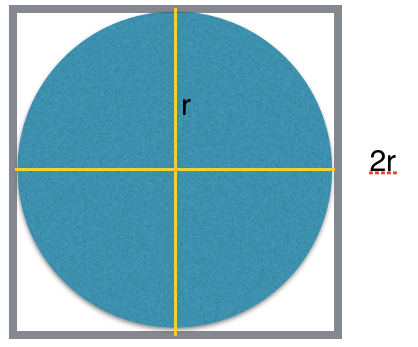
\includegraphics[scale=0.5]{Resources/Kolo_rysunek.png}
\caption{Koło o promieniu r wpisane w kwadrat - bok 2r.}
\end{figure}
Pole kwadratu przedstawionego na Rysunku 1 wynosi:
 \[(4\prod)^{2}\]
 natomiast koła oczywiście:
 \[(\prod)r^{2}\]
 \newpage
 Znając zatem pole koła jak i kwadratu można zauważyć że stosunek pola koła do pola kwadratu wynosi:
\[ \frac{PoleKola}{PoleKwadratu}=\frac{\prod r^{2}}{4r^{2} }= \frac{\prod}{4}\]
Następnie korzystając z tego, że pole koła jak i kwadratu zostały w jakiś sposób obliczone można wyciągnąć wzór na liczbę Pi:
\[\prod =4\frac{PoleKola}{PoleKwadratu}\]
Dojście do tego punktu mogłoby się wydawać zatoczeniem koła i powrotem do punktu początkowego problemu. Tak nie jest. Ponieważ dopiero w tym miejscu pojawia się cała charakterystyka metody Monte Carlo. Abstrakcyjnie należy sobię teraz wyobraźić sytuację, w której rzucamy bardzo dużo razy rzutkami w tarczę wyglądająca jak Rysunek 1. Kończąc grę, plansza będzie pokryta rzutkami znajdującymi sie we wnętrzu koła jak i poza nim na obszarze kwadratu. Podsumowując liczba rzutek w i poza kołem będzie równy stosunkowi pola koła do pola kwadratu.
\begin{figure}[h!]
\centering
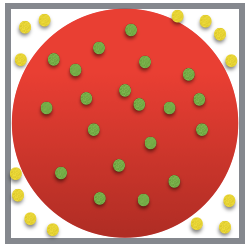
\includegraphics[scale=0.7]{Resources/Losowanie.png}
\caption{Przykład losowania punktów.}
\end{figure}
 Formalnie losowanie będzie odbywać się pośród punktów należących do zbioru pokrytego współrzędnymi należacymi do predziału [-2r,2r]. Stosunek liczby punktów
zawierających się w kole o środku w punkcie <0,0> i promieniu r do wszystkich wylosowanych punktów będzie dążył w nieskończoności (z pewnym prawdopodobieństwem) do stosunku tego pola koła do koła kwadratu o boku 2r. Co więcej, stosunek ten będzie identyczny również do ćwiartki koła. Jeżeli pole koła podzielimy na cztery i tak samo podzielimy pole kwadratu, to ich stosunek będzie wciąż taki sam. Oznacza to, że wystarczy, jeżeli będziemy losowali punkty o współrzędnych od 0 do r. Cała metoda sprowadza się więc do tego, by losować punkty, sprawdzać, czy mieszczą się w kole, i następnie podstawiać liczby wylosowanych punktów do wzoru. Losując odpowiednio dużo punktów, powinniśmy otrzymać z pewnym prawdopodobieństwem rozsądne przybliżenie liczby Pi.
\subsection{Implementacja algorytmu - program jednowątkowy.} 
Dla lepszego zrozumienia działania algorytmu i sprawdzenia jego rezultatów stworzony został program w języku C++ obliczający przybliżenie liczby Pi wykonujący wszystkie obliczenia szeregowo, czyli po prostu korzystający z jednego wątku. Program przyjmuje od użytkownika zadaną liczbę punktów. W rezultacie wyświetla obliczoną liczbę Pi oraz orginalne rozwinięcie.
\lstinputlisting[language=C++]{Code/obliczanie_pi.cpp}
\begin{figure}[h!]
\centering
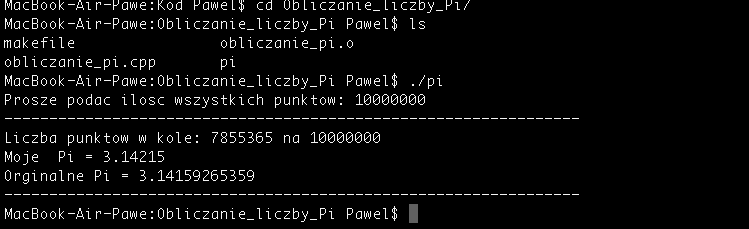
\includegraphics[scale=0.6]{Resources/Screen_Program_JedenWatek}
\caption{Przykład działania programu jednowątkowego.} 
\end{figure}
Jak widać na zamieszczonym zdjęciu ekranu program jednowątkowy obliczający rozwinięcie dziesiętne liczby Pi korzystając z metody Monte Carlo obliczył liczbę Pi równą 3.14215. Otrzymana dokładność sięga jedynie dwóch miejsc po przecinku przy stosunkowo już dużej ilości losowanych punktów - 10 mln. Program wyświetlił informację o tym, że 7855365 punktów znalazło się w kole.
\section{Zastosowane technologie.}
\subsection{Framework Django.}
\subsection{Technologia MPI.}
\subsection{CSS i HTML.}
\subsection{Komunikacja grupy.}
\subsubsection{GitHub.}
\subsubsection{Trello.}
\section{Plan realizacji.}
\subsection{Podział pracy między członków grupy.}
\subsection{Terminarz realizacji zadań.}
\section{Implementacja silnika obliczeniowego.}
\section{Aplikacja internetowa.}
\section{Testy.}
\section{Podsumowanie i wnioski.}

\end{document}
